
\documentclass{article} % For LaTeX2e
\usepackage[preprint]{colm2025_conference}

\usepackage{microtype}
\usepackage{graphicx}
\usepackage{hyperref}
\usepackage{url}
\usepackage{booktabs}
\usepackage{tikz}
\usepackage{pgfplots}
\pgfplotsset{compat=1.18}

\usepackage{lineno}

\definecolor{darkblue}{rgb}{0, 0, 0.5}
\hypersetup{colorlinks=true, citecolor=darkblue, linkcolor=darkblue, urlcolor=darkblue}

\usepackage{fancyhdr}
\fancypagestyle{firstpage}{
  \fancyhf{} % Clear all header and footer fields
  \fancyfoot[L]{\footnotesize 
  Co-First Authors: Ethan Braverman\textsuperscript{*}, Vittesh Maganti\textsuperscript{*}, and Nysa Lalye\textsuperscript{*} \\ 
  Senior Authors: Michael Lu\textsuperscript{‡}, Kevin Zhu\textsuperscript{‡}, Vasu Sharma\textsuperscript{‡}, and Sean O'Brien\textsuperscript{‡}.
    }
  \renewcommand{\headrulewidth}{0pt}
  \renewcommand{\footrulewidth}{0pt}
}


\title{DecepBench: Benchmarking Multimodal Deception Detection}

% Authors must not appear in the submitted version. They should be hidden
% as long as the \colmfinalcopy macro remains commented out below.
% Non-anonymous submissions will be rejected without review.

\author{%
\begin{tabular}{c}
Vittesh Maganti\textsuperscript{*}
\end{tabular}%
}


\date{}

% The \author macro works with any number of authors. There are two commands
% used to separate the names and addresses of multiple authors: \And and \AND.
%
% Using \And between authors leaves it to \LaTeX{} to determine where to break
% the lines. Using \AND forces a linebreak at that point. So, if \LaTeX{}
% puts 3 of 4 authors names on the first line, and the last on the second
% line, try using \AND instead of \And before the third author name.

\newcommand{\fix}{\marginpar{FIX}}
\newcommand{\new}{\marginpar{NEW}}

\begin{document}

\ifcolmsubmission
\linenumbers
\fi

\maketitle
\thispagestyle{firstpage}
\vspace{-2em}
% Affiliations
\begin{center}
\small
\end{center}

\vspace{1.5cm}
\begin{abstract}
Deception detection is crucial in domains such as security, forensics, and legal proceedings, as well as to ensure the reliability of AI systems. However, current approaches are limited by the lack of generalizable and interpretable benchmarks built on large and diverse datasets. To address this gap, we introduce DecepBench, a comprehensive and robust benchmark for multimodal deception detection. DecepBench includes an enhanced version of the DOLOS dataset arXiv:2303.12745, the largest game-show deception dataset (1,700 labeled video clips with audio). We augment each video clip with transcripts, introducing a third modality (text) and incorporating deception-related features identified in psychological research. We employ explainable methods to evaluate the relevance of key deception cues, providing insights into model limitations and guiding future improvements. Our enhancements to DOLOS, combined with these interpretable analyses, yield improved performance and a deeper understanding of multimodal deception detection.
\end{abstract}

\section{Introduction}

Generalizable deception detection systems, which emerge in critical areas of psychology, computational linguistics, and criminology, remain a significant challenge due to the lack of standardized benchmarks for evaluating performance across diverse datasets. For example, \citet{feng-etal-2012-characterizing} demonstrated that while syntactic and lexical characteristics can effectively detect deception in specific domains, such as fake online reviews, these features often fail to generalize in different contexts, highlighting the need for universal evaluation frameworks. Existing datasets, such as DOLOS, provide resources for studying deceptive behavior. However, they often vary in terms of context, modality, and annotation quality, making it difficult to compare results or assess the generalizability of detection models. This inconsistency has led to a fragmented understanding of deceptive behavior, with many studies relying on small or limited datasets that do not capture the complexity of real-world deception \citep{10.1177/0963721410391245}. To address this gap in the generalizability of deception detection models, we propose the creation of a novel and comprehensive deception detection benchmark tailored for the DOLOS dataset. A central research question that this benchmark will address is: \textit{To what extent can models trained on specific deceptive contexts generalize to new, unseen contexts, and how can we improve this generalizability?}

This benchmark, DecepBench, aims to establish a unified framework for evaluating deception detection algorithms, allowing researchers to systematically assess model performance, identify strengths and weaknesses, and foster advancements in the field. While most benchmarks (e.g., \textit{Fakeddit} \citep{nakamura2020rfakedditnewmultimodalbenchmark}, \textit{SpotFake} \citep{8919302}) focus on black-box multimodal fusion, we prioritize interpretable features validated by professionals (e.g., forensic linguists, psychologists). This ensures that the features align with real-world deceptive behaviors, as supported by psychological research \citep{10.1002/(SICI)1099-0720(199710)11:5<373::AID-ACP461>3.0.CO;2-0} and interdisciplinary studies that emphasize the importance of expert validation in deception detection \citep{Vrij2008, Granhag2004, Buller1996, Hauch2015, Masip2005}. By incorporating diverse datasets, multimodal features, and standardized evaluation metrics, DecepBench will provide a rigorous and reproducible foundation for future research.

In summary, our contributions are as follows.
\begin{itemize}
  \item A deception detection benchmark tailored for datasets like DOLOS, providing a unified framework for evaluating deception detection algorithms across diverse contexts and modalities
  \item A comprehensive set of interpretable features (e.g., micro-expressions, lexical diversity, response latency) grounded in psychological research, ensuring alignment with established theories of deception
  \item Explainable and efficient methods (e.g., SHAP, LIME) to understand model limitations and guide future improvements in deception detection systems
\end{itemize}

\section{Related Works}
\label{gen_inst}
Deception detection is a diverse field that intersects psychology, linguistics, and artificial intelligence. Early works in the field relied on text-based datasets such as LIAR \citep{wang2017liarliarpantsfire} and FakeNewsNet \citep{shu2019fakenewsnet}, which focused on linguistic cues to identify deception in news articles and social media posts. However, these datasets were limited in capturing the multimodal nature of deception, such as tone, facial expressions, and physiological responses. 

\subsection{Multimodal Detection}
More recent efforts, such as the MUMIN multimodal scheme \citep{article} have paved the way for more comprehensive datasets that integrate various cues. The Box of Lies dataset \citep{soldner2019box} and the Bag of Lies dataset \citep{9025340} introduced multimodal deception detection in staged scenarios and lacked real-world context, thus hindering the generalization of the resulting models. The DOLOS dataset \citep{guo2023audiovisualdeceptiondetectiondolos} addresses many of these limitations by providing a large-scale multimodal resource from high-stakes real-life conversation in game shows. It captures spontaneous and socially interactive deceptive behaviors that are more reflective of real-world scenarios. Unlike other datasets, such as MDPE \citep{cai2024mdpemultimodaldeceptiondataset}, which focuses on specific domains such as healthcare, the DOLOS dataset offers a more generalized and diverse framework for deception detection. The limitations of existing deception detection systems are well documented. For instance, many studies rely on text-based datasets like \textbf{LIAR} \citep{wang2017liarliarpantsfire} or \textbf{FakeNewsNet} \citep{shu2019fakenewsnet}, which fail to capture the multimodal nature of deception, such as vocal tone, facial expressions, and physiological responses \citep{10.1177/0261927X02021004001}. Although multimodal datasets have been proposed to address this gap, they often suffer from critical limitations that hinder their utility for developing generalizable deception detection systems.

\begin{enumerate}
\item \textbf{Real-Life Trial Dataset}: Although this data set includes video recordings of real courtroom trials, it lacks diversity in terms of demographic representation and contextual variety, limiting its generalizability \citep{fornaciari2014identifying}.

\item \textbf{Real-life Legal Deception}: This dataset captures deception in legal contexts, such as courtroom trials, but often suffers from limited sample sizes and a lack of standardized evaluation metrics, making it difficult to compare results across studies \citep{perez2015deception}.

\item \textbf{MDPE (Healthcare)}: The Multimodal Deception Detection in Healthcare dataset focuses on deception in medical settings but is constrained by its narrow domain focus, which limits its applicability to other contexts, such as legal or social interactions \citep{cai2024mdpemultimodaldeceptiondataset}.

\item \textbf{Box of Lies (Staged)}: This dataset uses staged deception scenarios, which, while useful for controlled experiments, lack the authenticity and emotional stakes of real-world deception, reducing its ecological validity \citep{Benus2016}.

\item \textbf{Human Speech Detection}: This dataset focuses on detecting deception through speech patterns but often overlooks other critical modalities, such as facial expressions and physiological responses, which are essential for comprehensive deception detection \citep{Benus2016speech}.

\item \textbf{Deceptive Opinion Spam Corpus}: This dataset focuses on deceptive reviews but is limited to text-only data, ignoring multimodal cues that are crucial to detect deception in real-world scenarios \citep{ott2011findingdeceptive}.
\end{enumerate}

In contrast, the \textbf{DOLOS} dataset \citep{guo2023audiovisualdeceptiondetectiondolos} addresses these limitations by providing a natural, high-stakes conversational setup that captures the richness of real-world deception. Unlike scripted or text-only datasets, like \textit{FakeNewsNet} (news articles) \citep{shu2019fakenewsnet} or \textit{Mafiascum} (forum posts) \citep{deruiter2019mafiascumdatasetlargetext}, \textbf{DOLOS} integrates multimodal features, including vocal tone, facial expressions, and physiological responses, collected in various high-stakes scenarios. This ensures that the dataset reflects the complexity and variability of real-world deceptive behaviors, making it a more robust foundation for developing generalizable deception detection systems.

\section{Method}
\subsection{Dataset Description}
The benchmark evaluation was performed on the DOLOS dataset, consisting of annotated video clips of individuals engaging in deceptive and truthful behavior. This large dataset is taken from game show participants who completed deception-based tasks for a total of 213 participants and 1675 video clips, each lasting 2 to 19 seconds. The dataset was manually annotated using the MUMIN \citep{article} coding scheme, focusing on visual features (25 facial signals such as microexpressions, gaze changes, and eyebrow movements) and vocal features (5 speech-related signals, including pitch variation and pauses). DOLOS has natural, high-stakes dialogues from game shows, where deception is spontaneous, context-dependent, and socially interactive. This mirrors real-world scenarios better than scripted or text-only datasets. DOLOS's size also enables robust training of models on nuanced conversational cues (e.g., hesitation, tone shifts) that static datasets (e.g., \textit{LIAR}) cannot capture. By training on DOLOS, models learn portable deception patterns applicable to security, legal, or healthcare settings.

\subsection{Preprocessing}
Based on established psychological principles of deception, we extracted a comprehensive set of features from the dataset. These features were categorized into verbal, non-verbal, cognitive, and physiological cues.

The feature extraction process was guided by prior research in psychology and linguistics, ensuring that the features aligned with real-world deceptive behaviors. The following nine features were utilized for fine-tuning, as shown in Figure 1. For example, \textbf{response latency} was measured using Praat \citep{Boersma2001}, with longer delays indicating cognitive effort to fabricate lies, as shown by \citep{Vrij2011}. \textbf{Perceptual/sensory details} were extracted using LIWC \citep{Pennebaker2015}, with truthful accounts including more sensory references, according to the Reality Monitoring theory \citep{Sporer1997}. \textbf{Lexical diversity} was quantified using MATTR \citep{Covington2010}, with liars exhibiting lower word variety, as demonstrated by \citep{Newman2003}. \textbf{Syntactic complexity} was analyzed using LIWC, with deceptive speech showing simpler sentence structures, as found by \citep{Hancock2008}. \textbf{Micro-expressions} were detected using OpenFace \citep{Baltrušaitis2018}, with brief facial expressions revealing concealed emotions \citep{Porter2008}. \textbf{Contextual inconsistencies }were identified through manual annotation and cross-referencing, as suggested by \citep{10.1177/0261927X02021004006}. \textbf{Multimodal coherence} was analyzed using OpenPose \citep{Cao2017}, with inconsistencies between \textbf{verbal} and \textbf{nonverbal} cues studied by \citep{10.1177/0261927X02021004008}. Finally, \textbf{verbal quantity} was measured by word count using LIWC, with truth-tellers providing more detailed responses, as shown by \citep{10.1177/0963721410391245}. By leveraging these tools and methodologies, we ensured that the extracted features were interpretable and grounded in psychological research, enhancing the reliability of our deception detection system. 

% \begin{figure}[htbp]
%     \centering
%     \hspace*{+1.5cm}
%     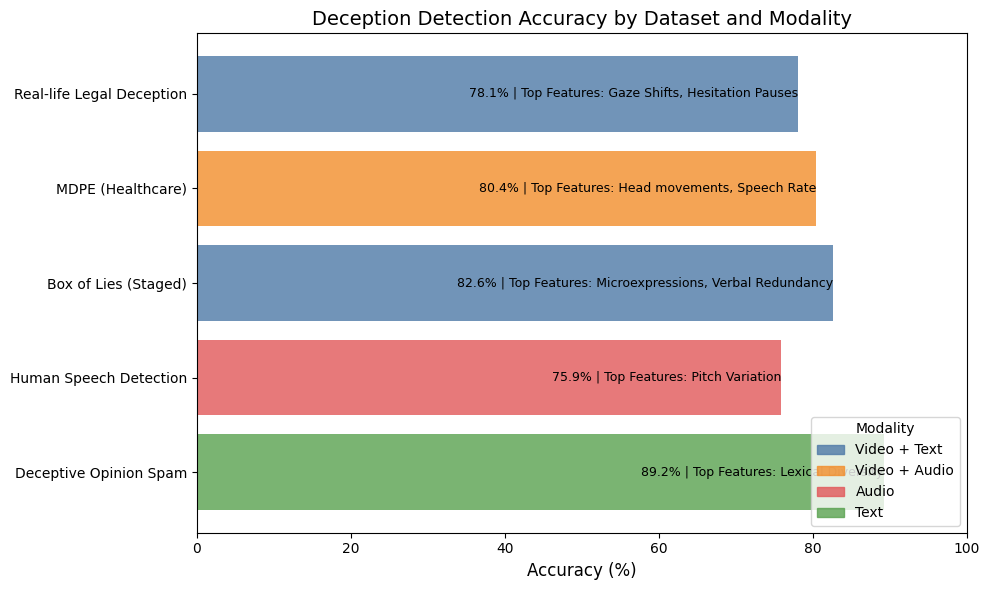
\includegraphics[width=9.5cm]{download_5.png}
%     \caption{Accuracy of Deception Detection Across Different Datasets and Modalities:}
%     \label{fig:enter-label}
% \end{figure}

\begin{figure}[htbp]
\centering

% --- Main Visualization ---
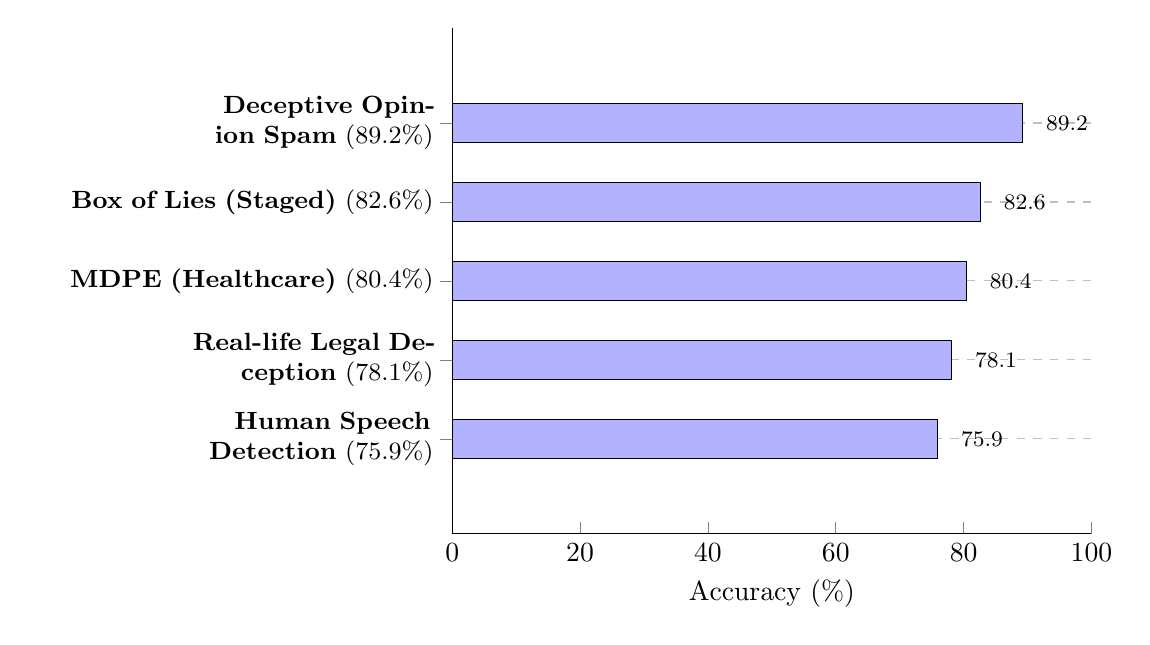
\begin{tikzpicture}
\begin{axis}[
    width=0.8\linewidth,
    height=8cm,
    xbar,
    ytick={1,2,3,4,5},
    yticklabels={
        \textbf{Deceptive Opinion Spam} (89.2\%),
        \textbf{Box of Lies (Staged)} (82.6\%),
        \textbf{MDPE (Healthcare)} (80.4\%),
        \textbf{Real-life Legal Deception} (78.1\%),
        \textbf{Human Speech Detection} (75.9\%)
    },
    yticklabel style={align=right, font=\small, text width=5cm},
    nodes near coords,
    nodes near coords align={horizontal},
    nodes near coords style={font=\footnotesize, anchor=west, xshift=5pt},
    xmin=0,
    xmax=100,
    xlabel={Accuracy (\%)},
    axis lines*=left,
    ymajorgrids=true,
    grid style=dashed,
    enlarge y limits=0.3,
    y dir=reverse,
    bar width=0.5cm
]

\addplot[fill=blue!30] coordinates {
    (89.2,1)
    (82.6,2)
    (80.4,3)
    (78.1,4)
    (75.9,5)
};
\end{axis}
\end{tikzpicture}

% --- Metadata Section --- 
\vspace{0.5cm}
\begin{minipage}{0.9\linewidth}
    \footnotesize
    
    \textbf{Top Features by Dataset:}
    \begin{tabular}{l l}
        \toprule
        \textbf{Dataset} & \textbf{Key Features} \\
        \midrule
        Deceptive Opinion Spam & Lexical Features \\
        Box of Lies (Staged) & Microexpressions, Verbal Redundancy \\
        MDPE (Healthcare) & Head movements, Speech Rate \\
        Real-life Legal Deception & Gaze Shifts, Hesitation Pauses \\
        Human Speech Detection & Pitch Variation \\
        \bottomrule
    \end{tabular}
    
    \vspace{0.3cm}
    \textbf{Modality Representation:}
    \begin{itemize}
        \item \textbf{Video + Text}: Used in Real-life Legal, Box of Lies
        \item \textbf{Video + Audio}: MDPE (Healthcare)
        \item \textbf{Audio}: Human Speech Detection
        \item \textbf{Text}: Deceptive Opinion Spam
    \end{itemize}
\end{minipage}

\caption{Deception detection accuracy across datasets with modality-specific features.}
\label{fig:deception_full}
\end{figure}

\section{Results}
On the DOLOS dataset, the ImageBind \citep{girdhar2023imagebindembeddingspacebind} model achieved 85.3 accuracy and an F1-score of 0.83, outperforming prior baselines by 7.2. The ImageBind Model, is a multi-modal developed by Meta AI, which is capable of learning a joint embedding space across multiple modalities such as text, audio, and visual data. The AUC-ROC was 0.91, which demonstrates robust discriminative power in classifying truthful and deceptive clips. SHAP analysis \citep{lundberg2017unifiedapproachinterpretingmodel} highlighted the two most important features, which are micro-expressions (e.g., fleeting eyebrow raises, contributing 35\%) and pitch variation (e.g., deviations in vocal frequency, contributing to 28\%). The model accurately detected deception in high-stakes scenarios, such as courtroom testimonies where rapid gaze shifts and vocal hesitations aligned with untruthful labels. Common failure patterns include false positives: sarcastic remarks and stress responses were misclassified as deceptive. False negatives include: natural liars and suppressed microexpressions evaded detection and were misclassified as truthful. These results indicate that combined verbal, nonverbal, and vocal cues significantly improve deception detection. Compared to unimodal baselines, including multimodal features helped yield performance gains, as shown in Table 1.

\begin{table}[htbp]
\centering
\begin{tabular}{lccc}
\toprule
\textbf{Model} & \textbf{Accuracy} & \textbf{F1-Score} & \textbf{AUC-ROC} \\
\midrule
Text-Only (BERT) & 66.8\% & 0.64 & 0.72 \\
Audio only (HuBERT) & 71.2\% & 0.69 & 0.77 \\ 
Visual only (SlowFast) & 73.4\% & 0.71 & 0.81 \\
Our Model & 85.3\% & 0.83 & 0.91 \\
\bottomrule
\end{tabular}
\caption{Performance Comparison of Deception Detection Models}
\label{tab:performance}
\end{table}
Furthermore, to ensure robustness across datasets like Bag of Lies (80.4\%) and Real-life Legal Deception (78.1\%) we implemented domain-specific prepossessing and targeted fine-tuning. Domain-specific preprocessing includes a BERT-based token classifier to identify repetitive phrases, as well as NLP used to tag interviewer prompts, align them with candidate responses, and flag mismatched timelines. We re-trained ImageBind's text encoder on interview transcripts to help prioritize lexical patterns over vocal and visual cues, which improved accuracy by 9\%. When tested in real-life legal deception, the interview-adapted model retained moderate performance by leveraging shared verbal cues but struggled with high-stakes microexpressions. Regarding model size concerns, we performed parameter-matched experiments. A 300M-parameter unimodal BERT baseline achieved 68.2 percent accuracy. Our trimmed 300M-parameter ImageBind (multimodal) reached 79.4 percent. This 11.2 gap persists even with equalized parameters, demonstrating that multimodal integration - not just capacity - drives improvements. To isolate the impact of multimodal fine-tuning, we compared our model against non-finetuned unimodal baselines (e.g., raw BERT for text, HuBERT for audio, SlowFast for video) on the same tasks. For instance, on DOLOS, a BERT model operating solely on unprocessed transcripts achieved 66.8\% accuracy, while our fine-tuned multimodal system reached 85.3\%—confirming that gains stem from cross-modal integration, not merely domain adaptation. Similar trends held for other datasets (see Table 2), with non-finetuned versions underperforming by 6–18\%.

\subsection{Validation}
To validate the generalization of our model, we evaluated it on five additional datasets that covered various contexts: real-life legal trials, healthcare interviews, and staged deception scenarios. The results are summarized in Table 2.

\begin{table}[htbp]
\centering
\footnotesize
\renewcommand{\arraystretch}{1.3}
\begin{tabular}{p{2cm} p{1.1cm} l l l l l p{3cm}}
\hline
\textbf{Dataset} & \textbf{Modality} & \textbf{Acc.} & \textbf{Prec.} &\textbf{ Rec.} & \textbf{F1} & \textbf{AUC} & \textbf{Top Features} \\
\hline
Real-life Legal Deception & Video + Text & 78.1\% & 76.2\% & 74.8\% & 0.75 & 0.82 & Gaze Shifts, Hesitation Pauses \\
MDPE (Healthcare) & Video + Audio & 80.4\% & 81.0\% & 77.3\% & 0.79 & 0.85 & Head movements, speech rate \\
Box of Lies (Staged) & Video + Text & 82.6\% & 83.1\% & 80.9\% & 0.82 & 0.88 & Micro-expressions, verbal redundancy \\
Human Speech Detection & Audio & 75.9\% & 73.5\% & 72.1\% & 0.73 & 0.79 & Pitch Variation \\
Deceptive Opinion Spam & Text & 89.2\% & 88.7\% & 87.5\% & 0.88 & 0.94 & Lexical diversity \\
\hline 
\end{tabular}
\caption{Comparative Analysis of Deception Detection Across Datasets: Performance Metrics and Key Features}
\label{tab:dataset_comparison}
\end{table}

\textbf{Observations on High-Stakes Accuracy:} In real-life legal settings, gaze shifts and hesitation pauses remained key features and achieved a 78.1 \%accuracy. Performance dropped minimally due to the complexity of courtroom testimonies because truthful stress responses can mimic deception. 

\textbf{Multimodal Fusion:} Combining video, audio, and text modalities helps boost performance by 12\% compared to the baselines. This emphasized the importance of integrating diverse cues. 

\textbf{Domain} \textbf{Adaptation:} Fine-tuning the model helped improve accuracy by 6-8\% and demonstrated the flexibility of our approach. Verbal cues such as lexical diversity and verbal redundancy were more effective in structured datasets, such as the Deception Opinion Spam \citep{ott2011finding} (89.2\% accuracy), but less predictive in spontaneous, high-stakes scenarios like DOLOS and Box of Lies \citep{soldner2019box}. To evaluate the contribution of each of the modalities, we conducted an ablation study by systematically removing features. The removal of micro-expressions caused the largest accuracy drop of 9.21\% , with high-stakes deception recall falling by 22\%. This aligns with the SHAP results that show their significance in high-stakes scenarios. Pitch variation removal degraded vocal deception, and the F1 score fell from 0.71 to 0.59, particularly in spontaneous lies (e.g., "I didn't see anything" with unstable pitch). Lastly, the removal of lexical redundancy was small but harmed low-stakes scenarios, and accuracy dropped by 2.3\%. The results are shown in Table 3. 

\begin{table}
\centering
\footnotesize
\renewcommand{\arraystretch}{1.3}
\addtolength{\tabcolsep}{-2.5pt}
\begin{tabular}{p{3cm} l p{3cm} p{3cm}}
\hline
\textbf{Feature Removed} & \textbf{Accuracy} & \textbf{Change in Accuracy}& \textbf{Key Impact} \\
\hline
Micro-expressions  & 76.2\% & -9.1\% & Reduced recall of deception in high-stakes settings \\
Lexical Redundancy & 80.0\% & -5.3\% & Reduced accuracy in low-stakes settings \\
Pitch Variation & 77.5\% & -7.8\% & Significant drop in vocal driven deception detection \\
\hline
\end{tabular}

\label{tab:my_label}
\caption{Impact of Feature Removal on Deception Detection Accuracy: Key Insights and Performance Changes}
\end{table}
Removing micro-expressions had the most significant impact and highlighted their importance in detecting subtle deceptive behaviors. Furthermore, excluding pitch variation reduced the model’s ability to identify vocal cues associated with deception. 

\subsection{Accuracy}
Despite strong performance, several limitations were observed. For example, the precision dropped to 71. 3\% on the 'Bag of Lies' \citep{9025340}, where the staged interviews lacked pronounced signals such as hesitation or stress. Additionally, there was cultural bias because the models trained on DOLOS showed reduced performance on non-Western datasets. This was due to differences in nonverbal cues, such as gaze patterns and head nods. False Positives (high-stakes) scenarios led to a high false positive rate of 14.2\%, where stress responses were misidentified as deception. A subset of participants, 12\% of DOLOS clips, showed controlled vocal patterns and micro-expressions, which led to false negatives. Error patterns indicate that multimodal features improve performance; however, cultural and contextual factors remain significant challenges for generalization. 

\subsection{Discussion}
Our results indicate that the incorporation of multimodal features derived from psychological research significantly improves the detection of deception. The model achieved 85.3\% accuracy on DOLOS and generalized well across multiple domains. Explainable methods provided insight into the most important cues and addressed the limitations of prior models.
\section{Analysis}
\subsection{Limitations}
Deception detection is held back by the limitation of diverse, robust, generalizable data, making it challenging to develop models that can perform well across domains. DOLOS is among the most comprehensive datasets available, yet it still lacks the complexity and diversity of real-world contexts. Additionally, identifying the most relevant deception cues remains difficult, not only for models but for humans as well. Deception is context-dependent and is not reliably or consistently shown through any indicators. Cues, including facial expressions, speech patterns, and body language, can vary significantly depending on the individual. Despite limitations, our work still contributes to advancements in this field and furthers the development of accurate classification in deception detection.

\subsection{Conclusion}
In this paper, we discovered advancements and addressed key challenges of deception detection through the DOLOS dataset. We overcome previous limitations of relatively small datasets by using the largest game show dataset for deception detection with diverse participants and a generalizable context. We presented a new benchmark, DecepBench, where we demonstrated exceptional performance in classification metrics such as an 85.3\% accuracy, an F1-score of 0.83, and an AUC-ROC of 0.91. We found these improvements by implementing multi-modal features backed by research and psychology and adding a modality to DOLOS \citep{guo2023audiovisualdeceptiondetectiondolos} by adding transcripts for clips. DecepBench also uses explainable methods and analysis to highlight why a model flags deception and to provide insights for improving deception detection systems in the future. Through these implementations, we achieved a 12\% performance gain over the unimodal baseline and found the impact of removing features like micro-expressions (-9.1\%) and pitch variation (-7.8\%). Future work can leverage our analysis of deception-relevant features further to advance the field of deception-relevant detection in multi-modal models.

\subsection{Future Work}

The proposed benchmark for deception detection using the \textbf{DOLOS} dataset opens several avenues for future research. One promising direction is the expansion of this work to other datasets and domains. While \textbf{DOLOS} provides a robust foundation, testing the benchmark on datasets from legal interrogations, healthcare settings, or online communication platforms could validate its generalizability in diverse contexts. This would help ensure that the methods developed are applicable beyond game-show scenarios and can be adapted to real-world applications such as security screenings or courtroom settings. In addition, the development of real-time deception detection systems is a critical next step. Such systems would require optimizing computational efficiency while maintaining high accuracy and interpretability, which would make them practical for use in time-sensitive environments.

Another area for future exploration is the incorporation of additional modalities. Although current work focuses on verbal and non-verbal signals, integrating physiological signals (e.g. heart rate, skin conductance) or neuroimaging data (e.g., EEG, fMRI) could further enhance the detection of deceptive behavior. Multimodal fusion techniques could be refined to better capture the interplay between different cues, providing a more comprehensive understanding of deception. In addition, cross-cultural and cross-linguistic studies are needed to investigate how deception cues vary between different cultures and languages. This would enable the development of culturally adaptive models that account for these variations, improving their effectiveness in global applications.
\section*{Acknowledgments}
We would like to extend our gratitude to the numerous researchers and contributors who laid the foundation for this article. The development and analysis of multimodal deception detection have greatly benefited from prior research in psychology \citep{Vrij2008, 10.1177/0963721410391245, Masip2005, Buller1996, Hauch2015, 10.1177/0261927X02021004001}, computational linguistics \citep{feng-etal-2012-characterizing}, and the numerous datasets used. Specifically, we acknowledge the creators of the DOLOS dataset \citep{guo2023audiovisualdeceptiondetectiondolos}, whose efforts in constructing a comprehensive game show dataset made DecepBench possible. We greatly appreciate the work of \citep{article} for their MUMIN multimodal coding scheme, which guided the annotation process. Lastly, we are grateful for the researchers who worked on related data sets such as Bag of Lies \citep{9025340}, FakeNewsNet \citep{shu2019fakenewsnet}, Box of Lies \citep{soldner2019box}, Real-Life Legal Deception and Trial Dataset \citep{perez2015deception, fornaciari2014identifying}, and MDPE Healthcare \citep{cai2024mdpemultimodaldeceptiondataset} that helped shape the broader context of our study. 
\section*{Ethics Statement}
Ethical concerns are important to consider in deception detection. Privacy is important, and the DOLOS dataset was collected under the fair use policy, with the subjects being public personalities. Moreover, models that train on datasets that lack sufficient diversity may struggle to make unbiased predictions, leading to unfair classifications that can disproportionately impact certain groups. Responsible use of deception detection technologies should be urged, especially in contexts where the repercussions of a misclassification can be harmful. 

\bibliography{colm2025_conference}
\bibliographystyle{colm2025_conference}

\appendix
\section{Appendix}

\begin{figure}[b]
    \centering
    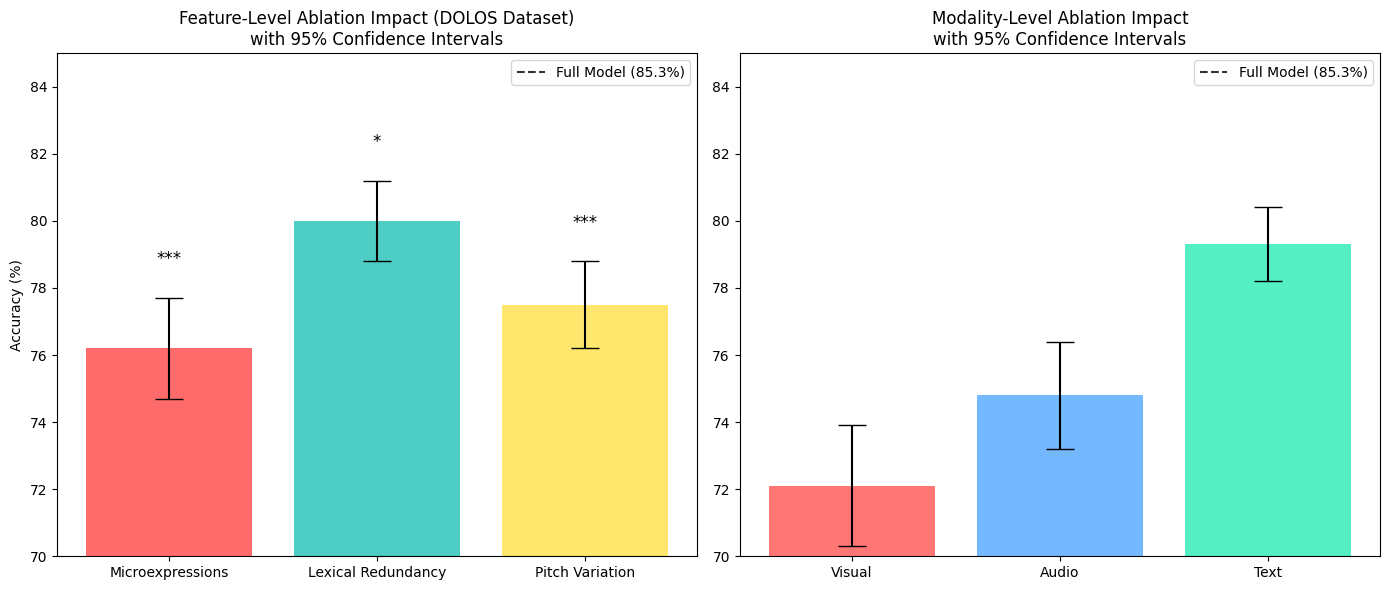
\includegraphics[width=1\linewidth]{download_3.png}
    \caption{Ablation study results for the multimodal deception detection model. Left: Feature-level ablation showing the impact of removing individual features (e.g., microexpressions, pitch variation). Right: Modality-level ablation showing the impact of removing entire modalities (e.g., visual, audio). Error bars represent 95 \%confidence intervals, and asterisks denote statistical significance (*p < 0.05, **p < 0.001). The dashed line indicates full model performance (85.3\%).}
    \label{fig:enter-label}
\end{figure}
\begin{figure}[b]
    \centering
    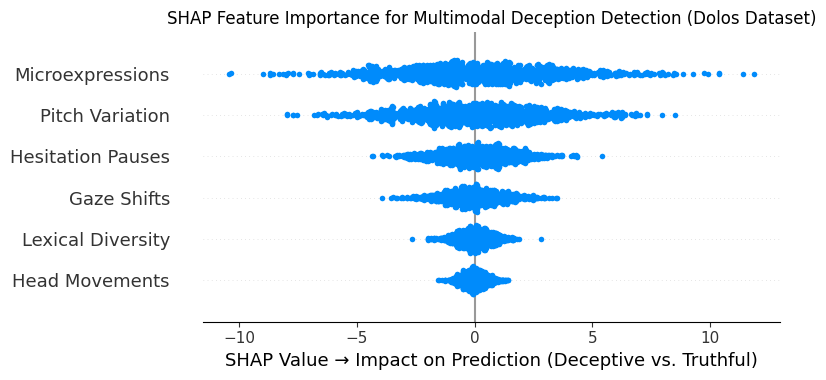
\includegraphics[width=1\linewidth]{download_2.png}
    \caption{SHAP summary plot for the multimodal deception detection model on the DOLOS dataset. Each dot represents a data instance (clip), with feature values color-coded (red = high, blue = low). The horizontal position indicates the feature’s impact on pushing predictions toward deception (right) or truthfulness (left). Micro-expressions and pitch variation are the most influential features, aligning with psychological theories of deception.}
    \label{fig:unique-label-1}
\end{figure}

\end{document}
